\documentclass{training}
\schoollogo{../../resources/intros/UX-05-sunday-night-movie.jpg}
\setlang{french}
\newcommand{\uxfond}{../../resources/fond/UX-05-sunday-night-movie.png}
% Filigrane PAR MODULE : \uxfond (PNG A4 dilue 30 %). Cadre noir vectoriel commun.
% Proportions original 744 px : marge 20/744, trait 1/744. Exterieur BLANC.
% Cadre via eso-pic +\put (coordonnees absolues) — pas de remember picture (decalage).
\usepackage{eso-pic}

\providecommand{\uxfond}{../../resources/fond/norme_fond_paliers_30.png}

\newlength{\uxmargin}
\newlength{\uxthick}
\newlength{\uxinnerw}
\newlength{\uxinnerh}
\setlength{\uxmargin}{0.02688\paperwidth}% 20/744
\setlength{\uxthick}{0.001344\paperwidth}% 1/744
\setlength{\uxinnerw}{\dimexpr\paperwidth-2\uxmargin-2\uxthick\relax}
\setlength{\uxinnerh}{\dimexpr\paperheight-2\uxmargin-2\uxthick\relax}

% Contenu strictement a l'interieur du trait (+ jour confortable).
\geometry{%
  includeheadfoot,
  left=22mm,
  right=22mm,
  top=20mm,
  bottom=18mm,
  headheight=30pt,
  headsep=5mm,
  footskip=12mm%
}

\AddToShipoutPictureBG{%
  \AtPageLowerLeft{%
    % Fond blanc page entiere
    \put(0,0){\color{white}\rule{\paperwidth}{\paperheight}}%
    % Filigrane module a l'interieur du cadre
    \put(\LenToUnit{\dimexpr\uxmargin+\uxthick\relax},\LenToUnit{\dimexpr\uxmargin+\uxthick\relax}){%
      \includegraphics[width=\uxinnerw,height=\uxinnerh]{\uxfond}}%
    % Cadre noir : bas, haut, gauche, droite
    \put(\LenToUnit{\uxmargin},\LenToUnit{\uxmargin}){%
      \color{black}\rule{\dimexpr\paperwidth-2\uxmargin\relax}{\uxthick}}%
    \put(\LenToUnit{\uxmargin},\LenToUnit{\dimexpr\paperheight-\uxmargin-\uxthick\relax}){%
      \color{black}\rule{\dimexpr\paperwidth-2\uxmargin\relax}{\uxthick}}%
    \put(\LenToUnit{\uxmargin},\LenToUnit{\uxmargin}){%
      \color{black}\rule{\uxthick}{\dimexpr\paperheight-2\uxmargin\relax}}%
    \put(\LenToUnit{\dimexpr\paperwidth-\uxmargin-\uxthick\relax},\LenToUnit{\uxmargin}){%
      \color{black}\rule{\uxthick}{\dimexpr\paperheight-2\uxmargin\relax}}%
  }%
}

\makeatletter
\fancyhf{}
\fancyheadoffset{0pt}
\renewcommand{\headrulewidth}{0pt}
\lhead{\parbox[t]{0.56\textwidth}{\RaggedRight\footnotesize\sloppy\@title}}
\rhead{\parbox[t]{0.36\textwidth}{\RaggedLeft\footnotesize\sloppy\@subtitle}}
\cfoot{\thepage}
% Coupures : underscore et slash dans les noms de fichiers / consignes
\DeclareRobustCommand{\_}{\textunderscore\allowbreak}
\makeatother

% Evite les depassements de longues lignes (Github, Name_FirstName_...)
\sloppy
\emergencystretch=3em
\hbadness=10000

% Sommaire type 42 : chapitres seulement
\setcounter{tocdepth}{0}
\renewcommand{\cftchappresnum}{}
\renewcommand{\cftchapaftersnum}{}
\setlength{\cftchapnumwidth}{2.0em}
\setlength{\cftbeforechapskip}{0.35em}
\cftsetindents{chapter}{0em}{2.0em}


\begin{document}

\title{Cinéma du dimanche soir}
\subtitle{Piscine UX/UI --- UX}
\member{Piscine UX/UI}{https://github.com/01-edu/UX-UI}
\summary{Un parcours, des wireframes, du mouvement, trois tests, une itération.}
\version{1.0}
\prerequisite{Le module précédent de cette piscine, ou aucun si c'est le premier.}
\maketitle

\newpage
\tableofcontents
\newpage


\chapter{Instructions}

L'avant-propos n'est pas un exercice. Il ne sera pas noté. Les exercices commencent au chapitre suivant, du contrat le plus simple au plus dur. Un exercice plus tardif n'est pas pris en compte si un plus tôt ne tient pas.

On ne regarde que ce qui est dans le répertoire de rendu de l'exercice. N'ajoutez pas un fichier que l'exercice ne nomme pas. Le nom d'un livrable suit le motif imprimé dans l'exercice : \texttt{Name\_FirstName\_DeliverableName\_Date\_VersionNumber}.

Le geste ne vous est pas donné. Les exemples d'un exercice portent parfois une contrainte que la phrase ne répète pas. Lisez-les. Vos autres références sont le manuel de l'outil choisi, la personne assise à côté, et les liens imprimés dans l'exercice.

L'ordre est celui de la quête. Sauter une étape parce qu'un écran plus tard semble plus intéressant produit un écran que personne ne sait expliquer.

\subsection*{Des images}

La marque en couverture est l'image de ce module. Les paliers pâles derrière le texte sont le fond de page. Ni l'un ni l'autre n'est un indice.

\subsection*{Des machines qui écrivent}

Vous pouvez vous servir d'un outil pour vérifier un mot, comme d'un dictionnaire. Vous ne pouvez pas remplacer un entretien, un test ou un fichier par un texte généré et le signer. Si vous ne pouvez pas montrer la personne, l'écran ou la ligne que vous avancez, l'exercice n'est pas fait.


\chapter{Avant-propos}

Saul Bass faisait faire aux génériques le travail d'une première scène (\emph{Autopsie d'un meurtre}, 1959, est l'exemple qu'on cite). Un dimanche soir devant un écran a le même contrat : la première minute doit dire où l'on est. Les exercices demandent de dessiner cette minute, puis de regarder quelqu'un la manquer.

\begin{center}
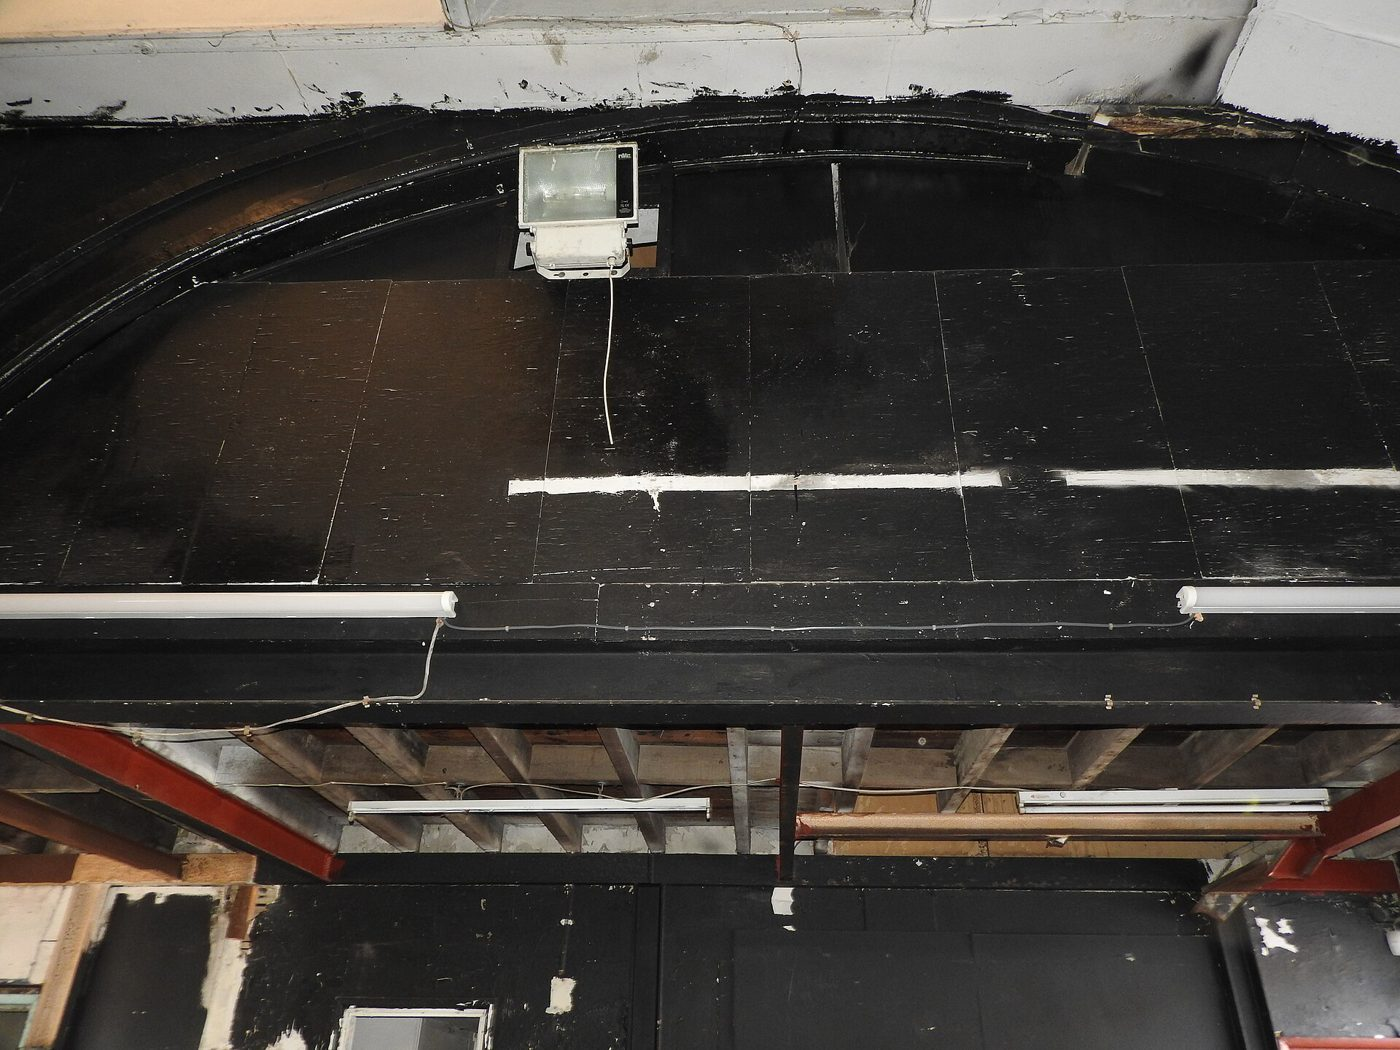
\includegraphics[width=0.78\textwidth,height=0.32\textheight,keepaspectratio]{../../resources/intros/UX-05-sunday-night-movie.jpg}\\[0.4em]
{\footnotesize Image : ClemRutter, CC BY-SA 4.0}
\end{center}

À regarder. Les vidéos sont un contexte. Elles ne sont pas le livrable.
\begin{itemize}
\item UX - Introduction \& Quest n°1, 01Edu \url{https://www.youtube.com/watch?v=UbE6WMeuvQg&list=PLHyAJ_GrRtf-RAtfngbRrFh1XDTnyXFDe}
\end{itemize}

\chapter{Exercice 00 : UX VI - Ex 1 - Parcours utilisateur}
\exnumber{00}
\extitle{UX VI - Ex 1 - Parcours utilisateur}
\exfiles{ex00/fichier Figma, nomme Name\_FirstName\_DeliverableName\_Date\_VersionNumber}
\exauthorize{Those named in the exercise}
\makeheaderfiles

\textbf{Contexte :}

Your company's client is a movie theaters chain called, Movie 4 all.

They want to launch a platform for people who want to watch movies but don't want to spend endless time selecting one.
You are replacing someone in the company who has already worked on the user research, the problem statement and the list of features they plan to develop. Your goal is to prototype and test these features.

\textbf{Instructions :}

Based on the 3 features that have come out of the ideation workshops led by your collegues, design 3 user flows (1 per feature).

Features:

\begin{itemize}
\item 1: Adding a filter based on their current mood
\item 2: Offer a selection of 3 movies to be watched
\item 3: Ask users to rate the movie after watching it for further recommendation
\end{itemize}

\textbf{Livrables :}

\begin{itemize}
\item 3 user flows on a board (digital or pictures of a paper board)
\item Déposez les documents sur Github, dans un zip nommé « ProjectTitle\_Name\_FirstName », et chaque livrable ainsi : « Name\_FirstName\_DeliverableName\_Date\_VersionNumber ». Exemple : « Doe\_John\_MidFiPrototype\_05242024\_V1 ».
\item Ajoutez un titre dans tous les documents écrits.
\item Soignez l'aspect global des livrables. Ils doivent être clairs, simples et lisibles. Vous pouvez regarder canva.com, sans surcharger le dessin de détails.
\end{itemize}

\textbf{Ressources :}

\begin{itemize}
\item User flow glossary \url{https://www.productplan.com/glossary/user-flow/}
\item Site flows vs User Flows \url{https://uxmovement.com/wireframes/site-flows-vs-user-flows-when-to-use-which/}
\item How to make a User Flow diagram \url{https://www.lucidchart.com/blog/how-to-make-a-user-flow-diagram}
\end{itemize}

\textbf{Outils recommandés :}

\begin{itemize}
\item Figma
\item Whimsical
\end{itemize}


\chapter{Exercice 01 : UX VI - Ex 2 - Wireframes}
\exnumber{01}
\extitle{UX VI - Ex 2 - Wireframes}
\exfiles{ex01/fichier Figma, nomme Name\_FirstName\_DeliverableName\_Date\_VersionNumber}
\exauthorize{Those named in the exercise}
\makeheaderfiles

\textbf{Instructions :}

Based on the 3 user flows, design 3 series of wireframes.

\textbf{Livrables :}

\begin{itemize}
\item 3 series of wireframes (6 to 12 screens per flow) on Figma
\item Déposez les documents sur Github, dans un zip nommé « ProjectTitle\_Name\_FirstName », et chaque livrable ainsi : « Name\_FirstName\_DeliverableName\_Date\_VersionNumber ». Exemple : « Doe\_John\_MidFiPrototype\_05242024\_V1 ».
\item Soignez l'aspect global des livrables. Ils doivent être clairs, simples et lisibles. Vous pouvez regarder canva.com, sans surcharger le dessin de détails.
\end{itemize}

\textbf{Pistes :}

\begin{itemize}
\item Drawing paper prototypes before going digital might save you some time ;)
\item Vocabulary
\begin{itemize}
\item Basse fidélité : prototypes papier - exemple \url{https://miro.medium.com/max/1400/1*5nUfqqA2gjdAYHagjbHA5w.jpeg}
\item Moyenne fidélité : wireframes, noir et blanc, seulement les éléments principaux, sur un outil de prototype - exemple \url{https://miro.medium.com/max/1400/1*eGSfaxwYbxUFomYbyO6GWw.png}
\item Haute fidélité : wireframes avec couleur, styles, détails graphiques et micro-interactions - exemple \url{https://miro.medium.com/max/1400/1*Xn0HSKAvhr4TZzC9lN5udw.gif}
\end{itemize}
\end{itemize}

\textbf{Ressources :}

\begin{itemize}
\item How to start sketching and wireframing \url{https://uxdesign.cc/how-to-start-sketching-and-wireframing-84a821f092e2}
\item Why should product teams use wireframes more often? \url{https://uxdesign.cc/why-should-product-teams-use-wireframes-more-often-60e34a2bc55}
\item The 5-pass reduction wireframing: A minimalist UX technique \url{https://uxdesign.cc/the-5-pass-reduction-wireframing-a-minimalist-ux-technique-aa415aad9ce2?sk=a218ac4db9d1049249bd381fbc5edeee}
\item The art of designing good wireframes \url{https://uxdesign.cc/the-art-of-designing-good-wireframes-8a2a9c10a95b}
\end{itemize}

\textbf{Outils recommandés :}

\begin{itemize}
\item Figma
\end{itemize}

\textbf{Citation :}

'77\% of users return to content and information sites because of ease-of-use. Only 22\% return because the site belongs to a favorite brand.' Forrester


\chapter{Exercice 02 : UX VI - Ex 3 - Animation des wireframes}
\exnumber{02}
\extitle{UX VI - Ex 3 - Animation des wireframes}
\exfiles{ex02/fichier Figma, nomme Name\_FirstName\_DeliverableName\_Date\_VersionNumber}
\exauthorize{Those named in the exercise}
\makeheaderfiles

\textbf{Instructions :}

Animate your wireframes on Figma.

Think about multistate!!

Cet exercice se fait seul.

\textbf{Livrables :}

\begin{itemize}
\item An animated prototype on Figma
\item Déposez le fichier Figma sur Github, nommé ainsi : « Name\_FirstName\_DeliverableName\_Date\_VersionNumber ». Exemple : « Doe\_John\_MidFiPrototype\_05242024\_V1 ».
\item Ajoutez un titre dans le fichier.
\item Soignez l'aspect global du fichier. Il doit être clair, simple et lisible. Vous pouvez regarder canva.com, sans surcharger le dessin de détails.
\end{itemize}

\textbf{Ressources :}

\begin{itemize}
\item Efficiently Manage Your Designs - How Mockplus State Page Helps To View \& Manage Multiple State \url{https://help.mockplus.com/p/372}
\end{itemize}


\chapter{Exercice 03 : UX VI - Ex 4 - Test de la fonction 1}
\exnumber{03}
\extitle{UX VI - Ex 4 - Test de la fonction 1}
\exfiles{ex03/archive zip, nomme Name\_FirstName\_DeliverableName\_Date\_VersionNumber}
\exauthorize{Ceux nommés dans l'exercice}
\makeheaderfiles

\textbf{Instructions :}

Testez vos wireframes !

Concentrez-vous sur le 1er parcours. Préparez un protocole de test avec vos objectifs de recherche (ce que vous voulez tester), testez-le auprès de 5 personnes différentes et notez 3 façons d'améliorer le prototype.

\textbf{Livrables :}

\begin{itemize}
\item Un PDF avec un protocole de test
\item Des photos des tests en cours
\item Un PDF avec 3 idées pour améliorer le prototype d'après les retours.
\item Déposez les documents sur Github, dans un zip nommé « ProjectTitle\_Name\_FirstName », et chaque livrable ainsi : « Name\_FirstName\_DeliverableName\_Date\_VersionNumber ». Exemple : « Doe\_John\_MidFiPrototype\_05242024\_V1 ».
\item Ajoutez un titre dans tous les documents écrits.
\item Soignez l'aspect global des livrables. Ils doivent être clairs, simples et lisibles. Vous pouvez regarder canva.com, sans surcharger le dessin de détails.
\end{itemize}

\textbf{Ressources :}

\begin{itemize}
\item Comment mener un entretien utilisateur (tutoriel de Google Ventures) \url{https://www.youtube.com/watch?v=Qq3OiHQ-HCU}
\item Mener un test d'utilisabilité \url{https://www.usability.gov/how-to-and-tools/methods/running-usability-tests.html}
\item Tests d'utilisabilité : qu'est-ce que c'est et comment les faire ? \url{https://uxdesign.cc/usability-testing-what-is-it-how-to-do-it-51356e5de5d}
\item Analyser les données de tests d'utilisabilité \url{https://uxdesign.cc/analysing-usability-testing-data-97667ae4999e}
\item L'art du guerrilla usability testing \url{http://www.uxbooth.com/articles/the-art-of-guerrilla-usability-testing/}
\item Comment rédiger un rapport de tests utilisateurs que les gens liront vraiment \url{https://uxdesign.cc/how-to-write-a-user-testing-report-that-people-will-actually-read-652d15d2f92e}
\end{itemize}


\chapter{Exercice 04 : UX VI - Ex 5 - Test de la fonction 2}
\exnumber{04}
\extitle{UX VI - Ex 5 - Test de la fonction 2}
\exfiles{ex04/archive zip, nomme Name\_FirstName\_DeliverableName\_Date\_VersionNumber}
\exauthorize{Those named in the exercise}
\makeheaderfiles

\textbf{Instructions :}

Testez vos wireframes !

Focus on the 2nd journey. Prepare a test protocol with your research goals (what you want to test), test it on 5 different people and write down 3 ways to improve the prototype.

\textbf{Livrables :}

\begin{itemize}
\item Un PDF avec un protocole de test
\item Des photos des tests en cours
\item Un PDF avec 3 idées pour améliorer le prototype d'après les retours.
\item Déposez les documents sur Github, dans un zip nommé « ProjectTitle\_Name\_FirstName », et chaque livrable ainsi : « Name\_FirstName\_DeliverableName\_Date\_VersionNumber ». Exemple : « Doe\_John\_MidFiPrototype\_05242024\_V1 ».
\item Ajoutez un titre dans tous les documents écrits.
\item Soignez l'aspect global des livrables. Ils doivent être clairs, simples et lisibles. Vous pouvez regarder canva.com, sans surcharger le dessin de détails.
\end{itemize}

\textbf{Ressources :}

\begin{itemize}
\item How to do a user interview (tutorial from Google Ventures) \url{https://www.youtube.com/watch?v=Qq3OiHQ-HCU}
\item Running a usability test \url{https://www.usability.gov/how-to-and-tools/methods/running-usability-tests.html}
\item Usability testing: what is it and how to do it? \url{https://uxdesign.cc/usability-testing-what-is-it-how-to-do-it-51356e5de5d}
\item Analyzing usability testing data \url{https://uxdesign.cc/analysing-usability-testing-data-97667ae4999e}
\item The art of guerrilla usability testing \url{http://www.uxbooth.com/articles/the-art-of-guerrilla-usability-testing/}
\item How to write a user testing report that people will actually read \url{https://uxdesign.cc/how-to-write-a-user-testing-report-that-people-will-actually-read-652d15d2f92e}
\end{itemize}


\chapter{Exercice 05 : UX VI - Ex 6 - Test de la fonction 3}
\exnumber{05}
\extitle{UX VI - Ex 6 - Test de la fonction 3}
\exfiles{ex05/archive zip, nomme Name\_FirstName\_DeliverableName\_Date\_VersionNumber}
\exauthorize{Those named in the exercise}
\makeheaderfiles

\textbf{Instructions :}

Testez vos wireframes !

Focus on the 3rd journey. Prepare a test protocol with your research goals (what you want to test), test it on 5 different people and write down 3 ways to improve the prototype.

\textbf{Deliverables}:

\begin{itemize}
\item Un PDF avec un protocole de test
\item Des photos des tests en cours
\item Un PDF avec 3 idées pour améliorer le prototype d'après les retours.
\item Déposez les documents sur Github, dans un zip nommé « ProjectTitle\_Name\_FirstName », et chaque livrable ainsi : « Name\_FirstName\_DeliverableName\_Date\_VersionNumber ». Exemple : « Doe\_John\_MidFiPrototype\_05242024\_V1 ».
\item Ajoutez un titre dans tous les documents écrits.
\item Soignez l'aspect global des livrables. Ils doivent être clairs, simples et lisibles. Vous pouvez regarder canva.com, sans surcharger le dessin de détails.
\end{itemize}

\textbf{Resources}:

\begin{itemize}
\item How to do a user interview (tutorial from Google Ventures) \url{https://www.youtube.com/watch?v=Qq3OiHQ-HCU}
\item Running a usability test \url{https://www.usability.gov/how-to-and-tools/methods/running-usability-tests.html}
\item Usability testing: what is it and how to do it? \url{https://uxdesign.cc/usability-testing-what-is-it-how-to-do-it-51356e5de5d}
\item Analyzing usability testing data \url{https://uxdesign.cc/analysing-usability-testing-data-97667ae4999e}
\item The art of guerrilla usability testing \url{http://www.uxbooth.com/articles/the-art-of-guerrilla-usability-testing/}
\item How to write a user testing report that people will actually read \url{https://uxdesign.cc/how-to-write-a-user-testing-report-that-people-will-actually-read-652d15d2f92e}
\end{itemize}


\chapter{Exercice 06 : UX VI - Ex 7 - Itération}
\exnumber{06}
\extitle{UX VI - Ex 7 - Itération}
\exfiles{ex06/archive zip, nomme Name\_FirstName\_DeliverableName\_Date\_VersionNumber}
\exauthorize{Ceux nommés dans l'exercice}
\makeheaderfiles

\textbf{Instructions :}

À partir de vos tests précédents, choisissez l'un de vos 3 prototypes.

Implémentez les 3 idées que vous avez notées comme suggestions.

Réalisez une autre série de tests (et adaptez votre protocole de test si nécessaire).

Rédigez un rapport avec les conclusions que vous avez tirées de cette boucle d'itération.

\textbf{Livrables :}

\begin{itemize}
\item Photos du nouveau test
\item Un rapport avec vos conclusions, vos impressions et vos apprentissages clés de cette itération (document PDF issu de Microsoft Word, Pages, Google Docs ou tout logiciel de traitement de texte)
\item Comparaison entre la V1 et la V2 du prototype dans le rapport
\item Déposez les documents sur Github, dans un zip nommé « ProjectTitle\_Name\_FirstName », et chaque livrable ainsi : « Name\_FirstName\_DeliverableName\_Date\_VersionNumber ». Exemple : « Doe\_John\_MidFiPrototype\_05242024\_V1 ».
\item Ajoutez un titre dans tous les documents écrits.
\item Soignez l'aspect global des livrables. Ils doivent être clairs, simples et lisibles. Vous pouvez regarder canva.com, sans surcharger le dessin de détails.
\end{itemize}

\textbf{Pistes :}

\begin{itemize}
\item Ce rapport sera remis au CEO. Soyez attentif aux détails et assurez-vous que le document est propre et facile à utiliser !
\end{itemize}


\end{document}
